\subsubsection{Memory Intensive}
\label{section:perf-memory}

\YIComment{Redo this}

\autoref{figure:memcpyw-mips} shows the performance of the \texttt{memcpyw(n)} test suite. This is the first test suite discussed where performance is not monotonic with regard to \texttt{n} and starts to rapidly fall as \texttt{n} is sufficiently increased.

This is because the more memory copied by the test, the more insertions and accesses are made to the internal hash table powering the memory map. Insertion and access time for the map implementation used becomes slower the more items present in the map \cite{tessil-benchmark}. This linear slowdown is true for all other major C++ unordered map implementations \cite{tessil-benchmark}. This slowdown affects both SUTs as they both internally use the same memory map.

Despite this continuous decrease in performance of the memory map, the overall emulator performance does not monotonically decrease and instead peaks. This is because, for low \texttt{n}, initialization and overhead costs are still being amortized, yielding a performance increase that outweighs the decrease in memory map performance. The JIT emulator has higher overhead costs and thus takes longer to peak. Overall the JIT emulator has higher performance once peaked due to its superior execution performance.

\begin{figure}[H]
    \centering
    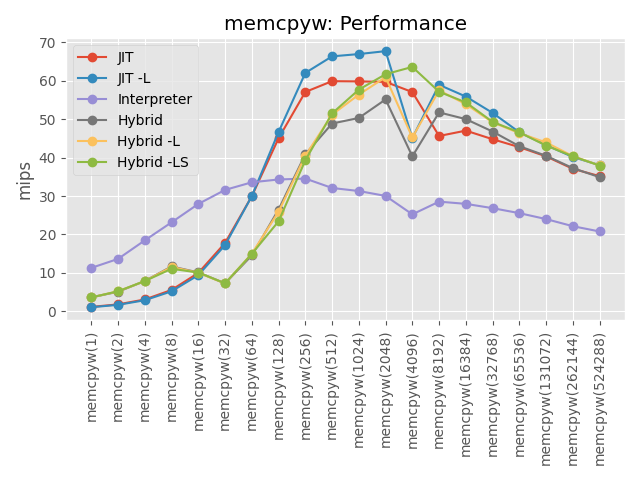
\includegraphics[scale=0.75]{output/graphs/tests/all/memcpyw/mips.png}
    \caption{Performance in mips of the memcpyw test suite.}
    \label{figure:memcpyw-mips}
\end{figure}